% !Mode\dots ``TeX:UTF-8''
% !TEX root = ../root.tex
\section{Algorithms for determining the online observability}
\label{sec:deter}
%After defining the online observability and comparing it with the existing four observability, we propose two algorithms to determine the online observability of \BCNs. Based on the definition of online observability, we propose the supertree to describe the process of determining the initial state of a \BCN. Then, we propose the algorithm to determine the online observability of \BCNs\ based on the supertree. But the supertree-based algorithm can not help us find all paths to determine the initial states of some \BCNs. In order to improve the shortcomings of the supertree-based algorithm, we propose the algorithm based on directed graph. Moreover, this algorithm can help us to do some optimizationin in the process of determining the initial state of a \BCN. But the algorithm based on directed graph may takes longer time for us to determine online observability of some \BCNs. 


\subsection{Input-labelled graph}
In this subsection, we define a directed graph for \BCN\ named input-labelled graph. Based on the input-labelled graph and the way to construct it, we propose determination algorithm for online observability in the following subsection.

\begin{definition}[Input-labelled Graph]
Let $V$, $E$ and $L$ be the vertex set, the edge set and the labelling function of an input-labelled graph $G=(V, E, L)$. $G$ is called the input-labelled graph of the \BCN\, if 
\begin{itemize}
\item  $V=\{\mathsf{S}\in\bigcup_{j=1}^{(2^m -1)} 2^{\Ded(\Delta_N,\varepsilon,\delta^j_{2^m} )}|$ there exists a $k\ge0$ such that $\mathsf{S}$ is $k$-step determinable$\}$;
\item  $E=\{(\mathsf{S}_1,\mathsf{S}_2)\in V\times V|$ there is an input $\mathsf{i} \in \Delta_M$ such that $|\Ded\left(\mathsf{S}_1,\mathsf{i},\varepsilon\right)|=|\mathsf{S}_1|$, and for every $\Ded(\mathsf{S}_1,\mathsf{i},\delta^j_{2^m})\neq \emptyset$ $\Ded(\mathsf{S}_1,\mathsf{i},\delta^j_{2^m})\in V$, $\mathsf{S}_2\subset\Ded(\mathsf{S}_1,\mathsf{i},\varepsilon)\}$;
\item  $L=\{E\mapsto 2^{\Delta_M}|(\mathsf{S}_1,\mathsf{S}_2)\mapsto\{\mathsf{i}\in \Delta_M|$$|\Ded\left(\mathsf{S}_1,\mathsf{i},\varepsilon\right)|=|\mathsf{S}_1|$, and for every $\Ded(\mathsf{S}_1,\mathsf{i},\delta^j_{2^m})\neq \emptyset$, $\Ded(\mathsf{S}_1,\mathsf{i},\delta^j_{2^m})\in V$, $\mathsf{S}_2\subset\Ded(\mathsf{S}_1,\mathsf{i},\varepsilon)\}\}$.
 \end{itemize}

\end{definition}

Comparing with supertree, in the directed graph, the states in the same node $\mathsf{S}^i$ with idential corresponding output. Thus, we do not need represent the processes of observing output by edges. And every node $\mathsf{S}^i$ appears only once, such that the directed graph has finite number of nodes. And then we can build the directed graph completely by $\Ded\left(\mathsf{S}^i,\mathsf{i}^{p},\mathsf{o}^{j}\right)$. Therefore, we use the directed graph to help us find all paths to determine the initial state of a \BCN.

From the {\em Lemma \ref{lemm:2}} in the {\em Section \ref{sec:online}}, we have that if for the set of states $\mathsf{S}^x$ there does not exist any $k^{1}\ge 0$ such that $\mathsf{S}^{x}$ is $k^{1}$-step determinable, and $\mathsf{S}^{x}\subseteq \mathsf{S}^{y}$. Then there does not exist any $k^{2}\ge 0$ that make $\mathsf{S}^{y}$ $k^{2}$-step determinable. Therefore, in the process of building the directed graph for a \BCN\ we build the nodes with fewer states at first, and then build the nodes with more states.
\begin{itemize}
\item  Because, once we can find node $\mathsf{S}^i$, such that there does not exist any $k^{i}\ge0$ makes $\mathsf{S}^{i}$ $k^{i}$-step determinable. And we know that there exists $\mathsf{o}^{j}\in \Delta_Q$ such that $\mathsf{S}^{i}\subseteq \Ded\left(\Delta_N,\varepsilon, \mathsf{o}^{j}\right)$. We have for $\Ded\left(\Delta_N,\varepsilon, \mathsf{o}^{j}\right)$, there does not exist any $k^{j}\ge 0$ that makes  $\Ded\left(\Delta_N,\varepsilon, \mathsf{o}^{j}\right)$ $k^{j}$-step determinable either, and then the \BCN\ is not online observable.
\item And as we determine the $k$-step determinability of every $\Ded(\mathsf{S},\mathsf{i}^{i},\mathsf{o}^{j})$, we can determine the $k$-step determinability of $\mathsf{S}$ easily.
\item  Finally, as the $k$-step determinability of the subsets of $\mathsf{S}$ has been checked, it is convenient for us to find the $\mathsf{i}^{i}$ which makes $\mathsf{S}$ $k$-step determinable by the subsets of $\mathsf{S}$.
 \end{itemize}
 \subsection{Determination algorithm}
With the input-labelled graph and the way to construct it. We propose the algorithm based on directed graph {\bf Algorithm~\ref{alg:1}}, and the {\bf Algorithm~\ref{alg:2}} to build nodes which is used in the {\bf Algorithm~\ref{alg:1}}.

\begin{itemize}
\item  Firstly, for every $w>0$ we try to build nodes with $w$ states, and the states with identical corresponding output. And we use the $NodeArray$ to represent them.
\item Secondly, if the nodes can  be built, when $w>1$, we check the determinability of every node and build edges for them. And, if we can not build any edge for one node, we have the \BCN\ is not online observable.
\item Fianlly, if we can not build any node with $w$ states, then we have the determinability of all of the set of states have been checked. Thus the \BCN\ is online observable, and {\bf Algorithm~\ref{alg:1}} returns the $\Delta_N$.
 \end{itemize}

\begin{algorithm}[h]
\caption{Algorithm based on directed graph}
\begin{algorithmic}[1]
\REQUIRE 
The updating rules of \BCN
\ENSURE  
The directed graph of \BCN
\STATE Bool ean value$Ob=$ true 
\STATE integer $i$ \
\STATE integer $j$ \
\STATE integer $w=1$
\STATE nodes $NodeArray[\ ]$
\STATE inputs $InputArray[\ ]$
\STATE {\sf buildnode}(w)
\STATE $w= w+1$
\STATE $NodeArray=${\sf buildnode}(w)
\WHILE {($NodeArray!=$Null)}
\FOR{($i=0$; $i<arraysize(NodeArray)$; $i++$)}
\IF{($p==2$)}
\STATE $InputArray$ = $\Delta_M$ 
\ELSE

\STATE Find $InputArray$ by other nodes

\ENDIF
\FOR{($j=0$; $j<arraysize(InputArray)$; $j++$)}
\STATE Check $NodeArray[i]$ by $InputArray[j]$ 
\STATE Build edges for $NodeArray[i]$ 
\ENDFOR
\IF {($NodeArray[i]$ has not any edge)}
\STATE  $Ob=$ false 
\STATE return Null
\ENDIF
\ENDFOR
\STATE $w= w+1$
\STATE $NodesArray=${\sf buildnode}(w)
\ENDWHILE
\STATE return $\Delta_N$\
\end{algorithmic}
 \label{alg:1}
\end{algorithm}
\begin{algorithm}[h!]
\caption{{\sf buildnode}(integer w)}
\begin{algorithmic}[1]
\REQUIRE 
The number of states $w$
\ENSURE  
The nodes with $w$ states which with the same corresponding outputs 
\STATE  Build all nodes with $w$ states 
\IF{(Failed to build)} 
\STATE  return Null
\ELSE 
\STATE  Classify these nodes
\STATE Sort the states in these nodes
\STATE Sort these nodes
\STATE return nodes
\ENDIF 
\end{algorithmic}
 \label{alg:2}
\end{algorithm}

There are some details in {\em Algorithm.\ref{alg:1}} and {\em Algorithm.\ref{alg:2}} are as follows:
\begin{itemize}
\item Build all nodes with $w$ states:
\begin{itemize}
\item Firstly, we classify all states by their corresponding outputs. Then we can get the set which contains all states with identical corresponding output i.e. $\Ded\left(\Delta_N,\varepsilon,\mathsf{o}^{j}\right)$.
\item Secondly, for every $\Ded\left(\Delta_N,\varepsilon,\mathsf{o}^{j}\right)$. If $w>|\Ded\left(\Delta_N,\varepsilon,\mathsf{o}^{j}\right)|$, then we could not get any set with $w$ states from $\Ded\left(\Delta_N,\varepsilon,\mathsf{o}^{j}\right)$. Else we can get $\frac{(|\Ded\left(\Delta_N,\varepsilon,o_j\right)|)!}{w!\times (|\Ded\left(\Delta_N,\varepsilon,o_j\right)|-w)!}$ sets of states, where $w!$ is the factorial of $w$.
\item Finally, we use all of the sets of states found in second step to build nodes. 
\end{itemize} 
 \item Sort the states in these nodes and sort these nodes: We sort the states inside the nodes at first, and then sort the nodes by the states of them. For example, in Fig.~\ref{fig:4} the nodes $\{\delta_{16}^0,\delta_{16}^1\}$, $\{\delta_{16}^0,\delta_{16}^2\}$ and $\{\delta_{16}^1,\delta_{16}^2\}$ are well shorted. 
  \item Find $InputArray$ by other nodes:
   For the node $NodeArray[i]$ contains $w$ sorted states, we can use the node with the first $(w-1)$ states of $\mathsf{S}^i$ and the node with the last $(w-1)$ states of $\mathsf{S}^i$ to find $InputArray$ for $NodeArray[i]$. For example, as shown in Fig.~\ref{fig:4} the set of edges from $\{\delta_{16}^0,\delta_{16}^1\}$ is $\{\delta_{4}^0,\delta_{4}^2,\delta_{4}^3\}$, and the set of edges from $\{\delta_{16}^1,\delta_{16}^2\}$ is $\{\delta_{4}^0,\delta_{4}^1,\delta_{4}^3\}$. And then, take the intersection of this two sets to be $InputArray$ of $\{\delta_{16}^0,\delta_{16}^1,\delta_{16}^2\}$ i.e. $InputArray=\{\delta_{4}^0,\delta_{4}^3\}$. 
  \item Check $NodeArray[i]$ by $InputArray[j]$:
     
\begin{itemize}
\item If $|\Ded\left(NodeArray[i],InputArray[j],\varepsilon\right)|<|NodeArray[i]|$, then the $InputArray[j]$ is a wrong input.
\item Else if every \[\Ded\left(NodeArray[i],InputArray[j],\mathsf{o}^{p}\right)\ne\emptyset\] already exists in the directed graph, and if $NodeArray[i]$ does not exist in the graph yet, we contruct it, and then connect it to every $\Ded\left(NodeArray[i],InputArray[j],\mathsf{o}^{p}\right)$ with the edge $InputArray[j]$.
\item Else if there exist a node \[\Ded\left(NodeArray[i],InputArray[j],\mathsf{o}^{p}\right)\ne\emptyset\] has not been constructed yet, then we check it latter. 
\end{itemize} 
\end{itemize} 

\begin{figure}[thpb]
      \centering
      \framebox{\parbox{3in}{
		\centerline{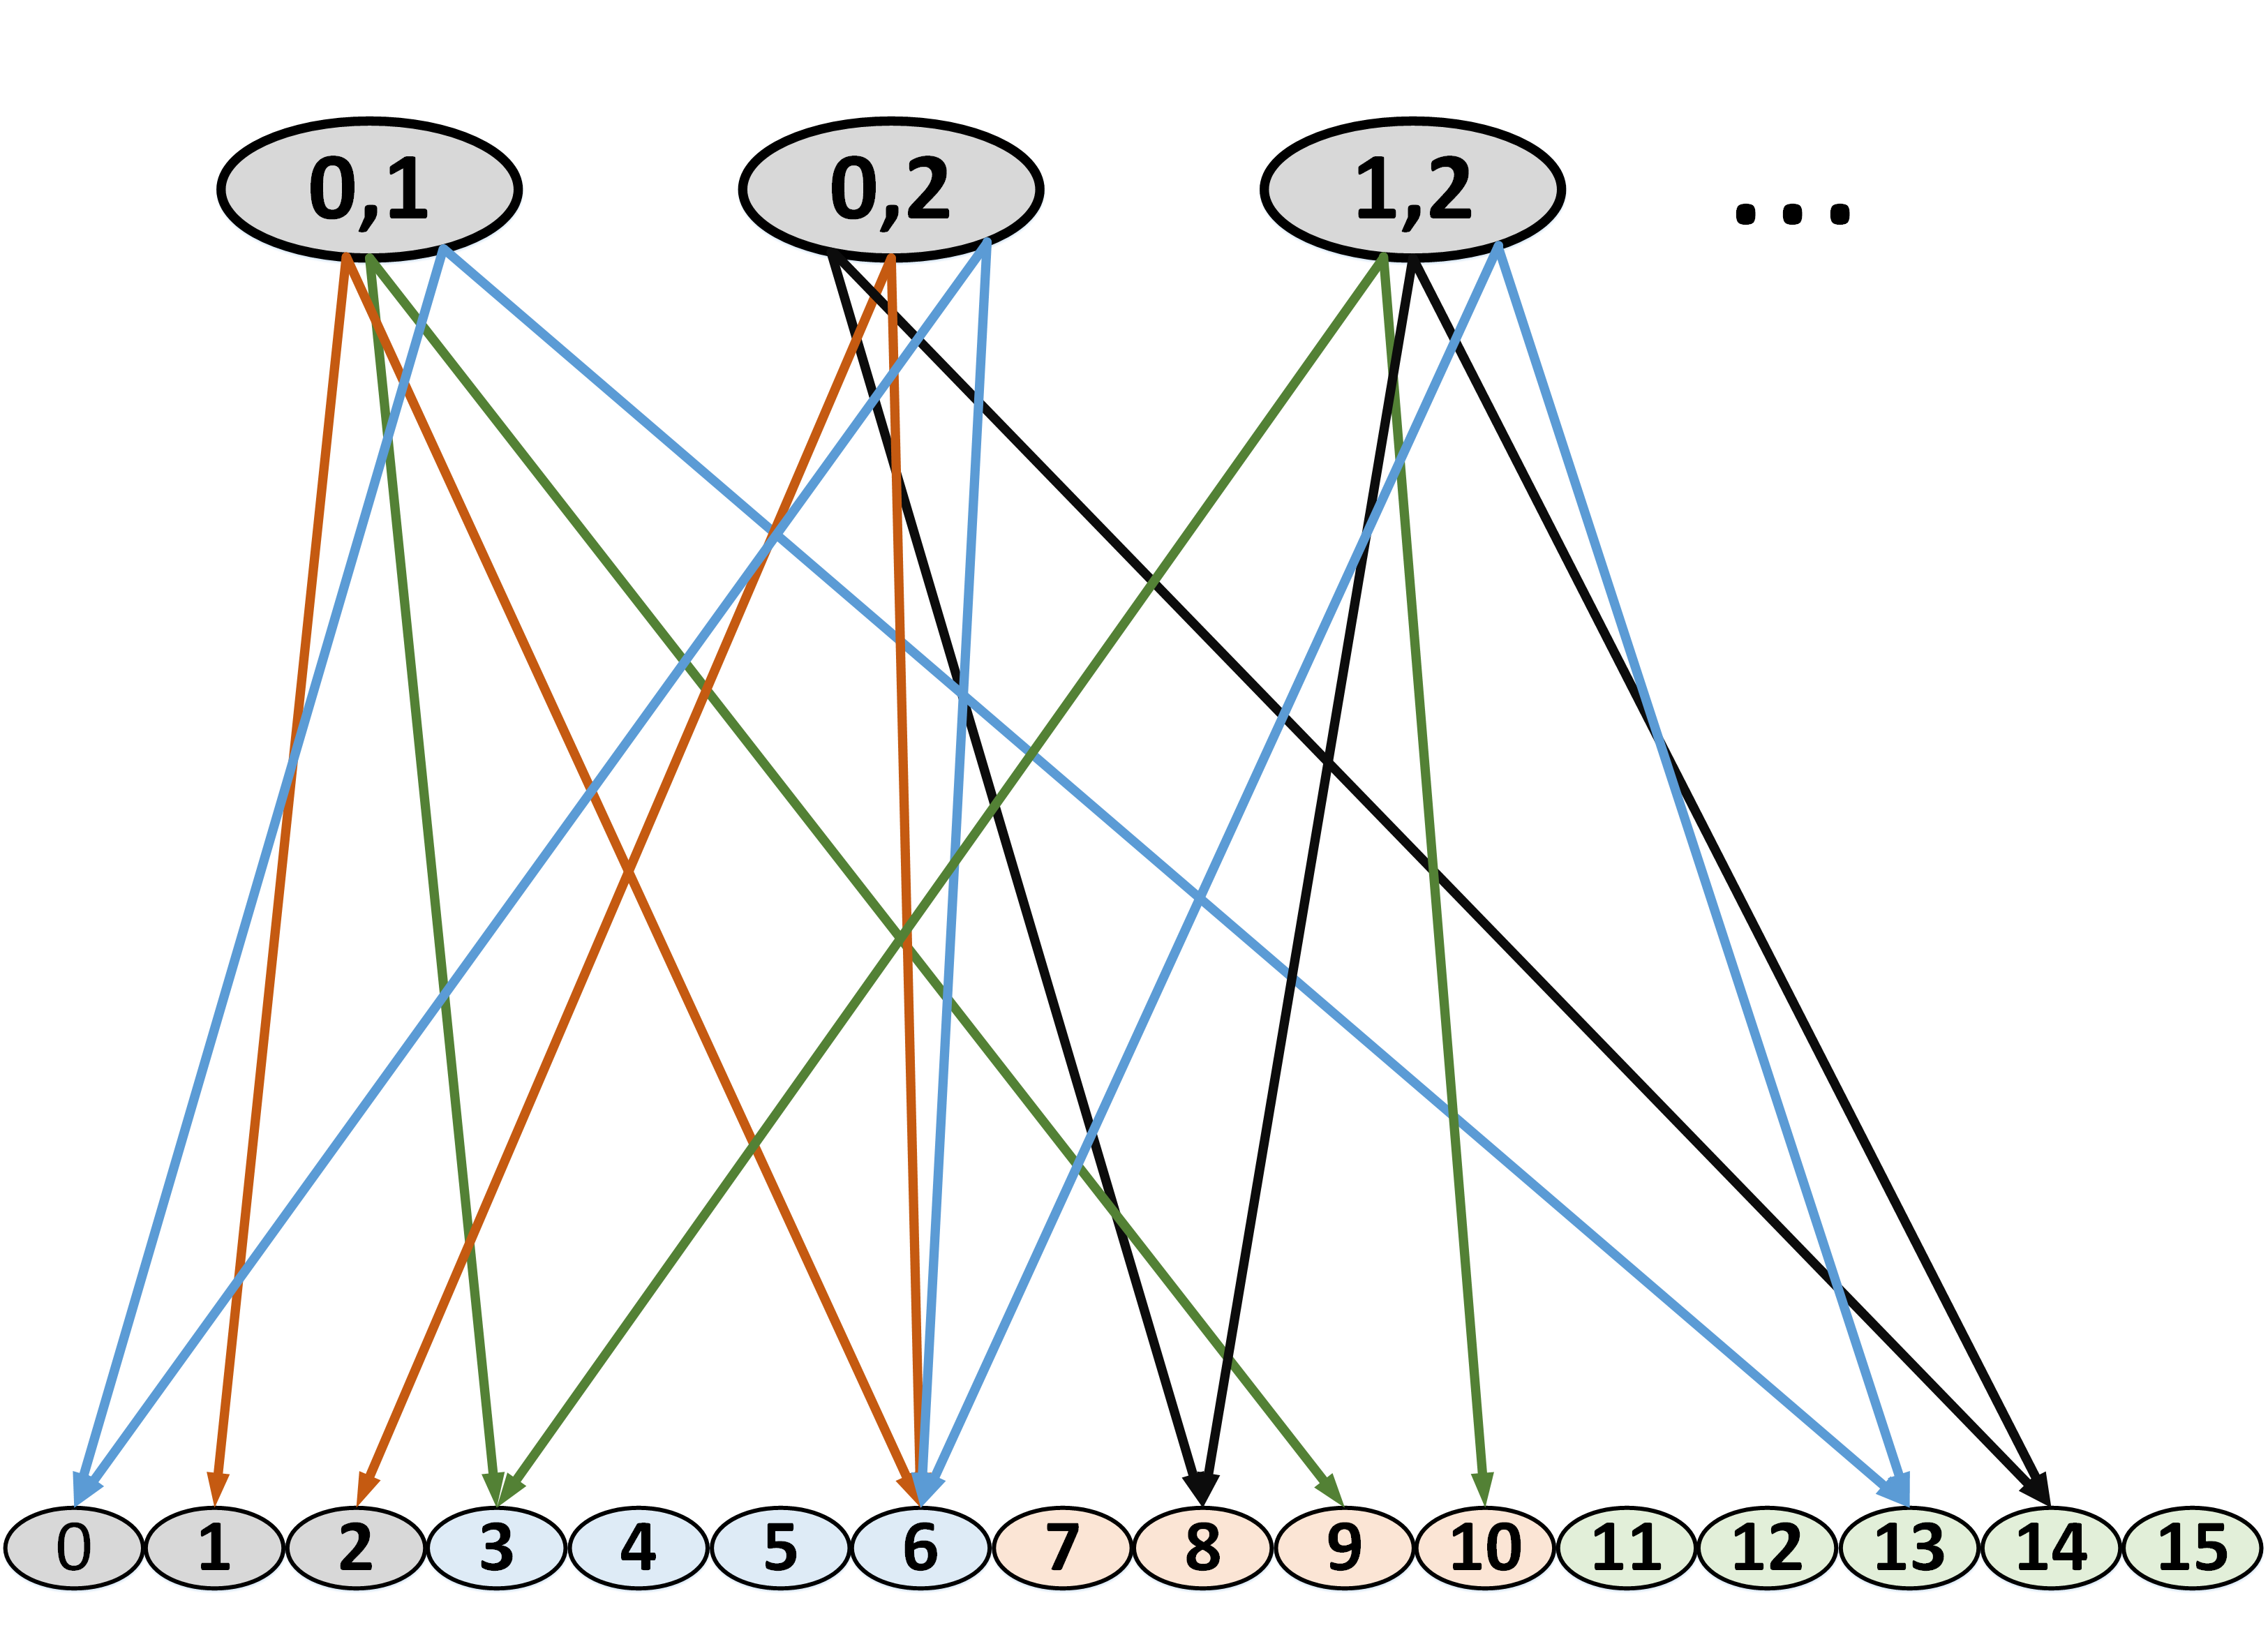
\includegraphics[scale=0.090]{figures/Fig4.png}}
	}}
      
      \caption{Part of the directed graph which represents $\{\delta_{16}^0,\delta_{16}^1\}$, $\{\delta_{16}^0,\delta_{16}^2\}$ and $\{\delta_{16}^1,\delta_{16}^2\}$. The green, black, orange, blue edges show the inputs $\delta_4^0$, $\delta_4^1$, $\delta_4^2$ and $\delta_4^3$ respectively.}
      \label{fig:4}
   \end{figure}

With the algorithm based on directed graph we can find all paths to determine the initial state of a \BCN. Thus, at time step $t$, we can use the $\mathsf{S}(t)$ and the directed graph to derive all of the input $\mathsf{i}(t)$ which can help us determine $\mathsf{s}(0)$. While, there comes a problem. Which input is the best input? To solve this problem, in the {\em Section \ref{sec:app}}, we will present how to decide the input to get better performance.
